\newcommand{\spywareTagResultsAucTable}{
    \begin{table}[H]
        \centering
        \begin{tabular}{|p{2,8cm}||P{2,4cm} P{2,4cm} P{2,4cm}|}
            \hline
            Spyware Tag & ALOHA\newline (M/B only) & ALOHA & Proposed\newline Model \\
            \hline
            AUC-ROC & - & 0.961$\pm$0.002 & 0.973$\pm$0.003 \\
            \hline
        \end{tabular}
        \caption[Spyware Tag prediction task AUC-ROC results]{AUC-ROC (Area Under Curve) of the different models for the \textbf{Spyware Tag} prediction task. Results were aggregated over \textBF{2} training runs with different weight initializations and minibatch orderings. Best results are shown in \textbf{bold}.} \label{tab:spywareTag_auc}
    \end{table}
}

\newcommand{\spywareTagResultsAtFprTable}{
    \begin{center}
        \begin{longtable}[c]{|P{3,2cm}||P{1,8cm} P{1,8cm} P{1,8cm} P{1,8cm} P{1,8cm}|}
            \hline
            Spyware Tag & \multicolumn{5}{c|}{{FPR}} \\
            & $10^{-5}$ & $10^{-4}$ & $10^{-3}$ & $10^{-2}$ & $10^{-1}$ \\
            \hline
            \endfirsthead

            \caption*{\raggedright ...continued from previous page} \\
            \hline
            Spyware Tag & \multicolumn{5}{c|}{\textbf{FPR}} \\
            & $10^{-5}$ & $10^{-4}$ & $10^{-3}$ & $10^{-2}$ & $10^{-1}$ \\
            \hline
            \endhead

            \caption*{\raggedleft ...continued on next page} \\
            \endfoot

            \caption[Spyware Tag prediction task results]{Mean and standard deviation results (TPR, Accuracy, Recall, Precision and F1-Score) of the different models for the \textbf{Spyware Tag} prediction task at different \textbf{FPR}s (\textit{False Positive Rates}). Results were aggregated over \textBF{2} training runs with different weight initializations and minibatch orderings. Best results are shown in \textbf{bold}. Under \textbf{TPR} results are also presented the percentage reduction in mean detection error and in ROC curve standard deviation introduced by the \textit{Proposed Model} with respect to both \textit{ALOHA} model and \textit{Joint Embedding}.} \label{tab:spywareTag_results_at_fpr} \\
            \endlastfoot

            \multicolumn{6}{|c|}{\textbf{TPR}} \\
            \hline
            ALOHA (M/B only) & - & - & - & - & - \\
            ALOHA & 0.113$\pm$0.002 & 0.187$\pm$0.074 & 0.190$\pm$0.074 & 0.599$\pm$0.027 & 0.899$\pm$0.002 \\
            Proposed Model & \textBF{0.132$\pm$0.126} & \textBF{0.406$\pm$0.001} & \textBF{0.504$\pm$0.006} & 0.713$\pm$0.004 & 0.918$\pm$0.001 \\
            \hline
            Error Reduction wrt\newline ALOHA (M/B only) & - & - & - & - & - \\
            Error Reduction wrt\newline ALOHA & 2.1\% & 26.9\% & 38.8\% & 28.4\% & 18.8\% \\
            \hline
            Std Reduction wrt\newline ALOHA (M/B only) & - & - & - & - & - \\
            Std Reduction wrt\newline ALOHA & -6200.0\% & 98.6\% & 91.9\% & 85.2\% & 50.0\% \\
            \hline
            \multicolumn{6}{|c|}{\textbf{Accuracy}} \\
            \hline
            ALOHA (M/B only) & - & - & - & - & - \\
            ALOHA & 0.905$\pm$0.000 & 0.913$\pm$0.008 & 0.913$\pm$0.008 & 0.948$\pm$0.003 & 0.900$\pm$0.000 \\
            Proposed Model & \textBF{0.907$\pm$0.013} & \textBF{0.936$\pm$0.000} & \textBF{0.946$\pm$0.001} & 0.960$\pm$0.000 & 0.902$\pm$0.000 \\
            \hline
            \multicolumn{6}{|c|}{\textbf{Recall}} \\
            \hline
            ALOHA (M/B only) & - & - & - & - & - \\
            ALOHA & 0.113$\pm$0.002 & 0.187$\pm$0.074 & 0.190$\pm$0.074 & 0.599$\pm$0.027 & 0.899$\pm$0.002 \\
            Proposed Model & \textBF{0.132$\pm$0.126} & \textBF{0.406$\pm$0.001} & \textBF{0.504$\pm$0.006} & 0.713$\pm$0.004 & 0.918$\pm$0.001 \\
            \hline
            \multicolumn{6}{|c|}{\textbf{Precision}} \\
            \hline
            ALOHA (M/B only) & - & - & - & - & - \\
            ALOHA & \textBF{1.000$\pm$0.000} & 0.997$\pm$0.000 & 0.953$\pm$0.017 & 0.877$\pm$0.005 & 0.518$\pm$0.001 \\
            Proposed Model & 0.994$\pm$0.006 & \textBF{0.998$\pm$0.000} & \textBF{0.984$\pm$0.000} & 0.895$\pm$0.000 & 0.523$\pm$0.000 \\
            \hline
            \multicolumn{6}{|c|}{\textbf{F1 Score}} \\
            \hline
            ALOHA (M/B only) & - & - & - & - & - \\
            ALOHA & 0.203$\pm$0.003 & 0.309$\pm$0.106 & 0.310$\pm$0.105 & 0.712$\pm$0.021 & 0.657$\pm$0.001 \\
            Proposed Model & \textBF{0.212$\pm$0.198} & \textBF{0.578$\pm$0.001} & \textBF{0.666$\pm$0.005} & 0.793$\pm$0.003 & 0.666$\pm$0.001 \\
            \hline
        \end{longtable}
    \end{center}
}

\newcommand{\spywareTagResultsSummaryTable}{
    \begin{table}[H]
        \centering
        \begin{tabular}{|P{3,2cm}||P{1,8cm} P{1,8cm} P{1,8cm} P{1,8cm} P{1,8cm}|}
            \hline
            \multicolumn{6}{|c|}{Spyware Tag (at FPR $=1\%$)} \\
            \hline
            Model & TPR & Accuracy & Precision & Recall & F1 score \\
            \hline
            ALOHA (M/B only) & - & - & - & - & - \\
            ALOHA & 0.599$\pm$0.027 & 0.948$\pm$0.003 & 0.877$\pm$0.005 & 0.599$\pm$0.027 & 0.712$\pm$0.021 \\
            Proposed Model & 0.713$\pm$0.004 & 0.960$\pm$0.000 & 0.895$\pm$0.000 & 0.713$\pm$0.004 & 0.793$\pm$0.003 \\
            \hline
        \end{tabular}
        \caption[Summary of Spyware Tag prediction task results]{Summary of the mean and standard deviation results of the different models for the \textbf{Spyware Tag} prediction task at \textbf{FPR} $=1\%$. Results were aggregated over \textBF{2} training runs with different weight initializations and minibatch orderings. Best results are shown in \textbf{bold}.} \label{tab:spywareTag_result_summary}
    \end{table}
}

\newcommand{\spywareTagRocAlohaMB}{
    \begin{figure}[H]
        \vspace*{-0.5cm}
        \centering
        \includegraphics[width=0.6\textwidth]{./results/spyware_tag_roc_alohaMB.png}
        \vspace*{-0.2cm}
        \caption[Spyware Tag prediction task ALOHA (M/B only) ROC curve]{ROC curve and AUC statistics of \textBF{ALOHA (M/B only)} model for the \textbf{Spyware Tag}. The line represents the \textit{mean} TPR at a given FPR, while the shaded region represents the \textit{standard deviation}. Statistics were computed over \textBF{2} training runs, each with random parameter initialization.}
        \label{fig:spywareTagRocAlohaMB}
    \end{figure}
}

\newcommand{\spywareTagRocAloha}{
    \begin{figure}[H]
        \vspace*{-0.5cm}
        \centering
        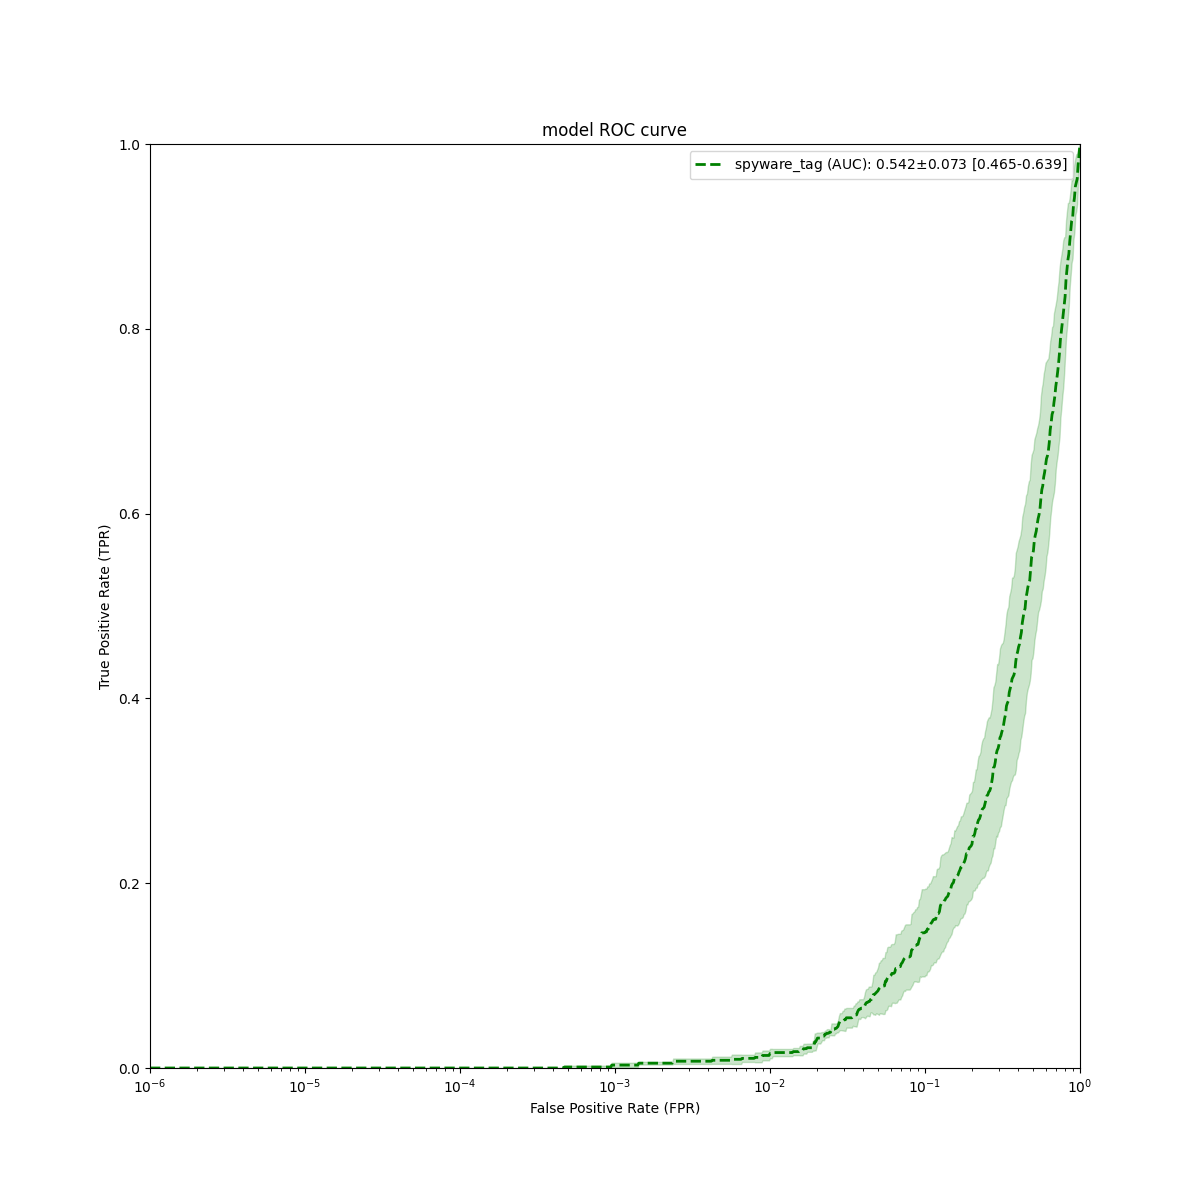
\includegraphics[width=0.6\textwidth]{./results/spyware_tag_roc_aloha.png}
        \vspace*{-0.2cm}
        \caption[Spyware Tag prediction task ALOHA ROC curve]{ROC curve and AUC statistics of \textBF{ALOHA} model for the \textbf{Spyware Tag}. The line represents the \textit{mean} TPR at a given FPR, while the shaded region represents the \textit{standard deviation}. Statistics were computed over \textBF{2} training runs, each with random parameter initialization.}
        \label{fig:spywareTagRocAloha}
    \end{figure}
}

\newcommand{\spywareTagRocProposedMethod}{
    \begin{figure}[H]
        \vspace*{-0.5cm}
        \centering
        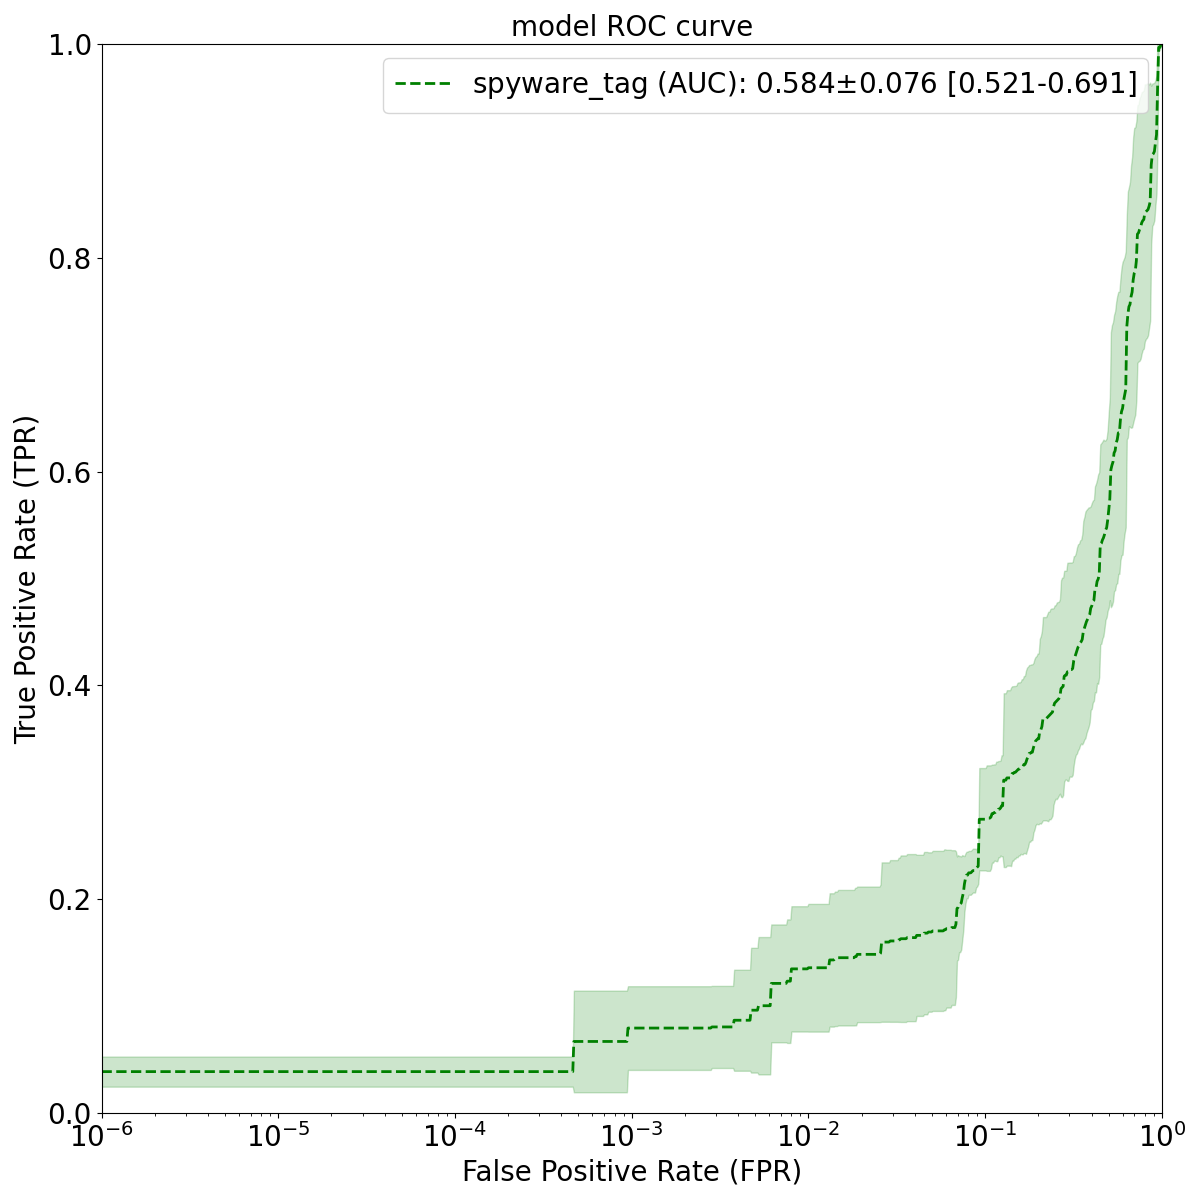
\includegraphics[width=0.6\textwidth]{./results/spyware_tag_roc_proposedModel.png}
        \vspace*{-0.2cm}
        \caption[Spyware Tag prediction task Proposed Model ROC curve]{ROC curve and AUC statistics of \textBF{Proposed Model} for the \textbf{Spyware Tag}. The line represents the \textit{mean} TPR at a given FPR, while the shaded region represents the \textit{standard deviation}. Statistics were computed over \textBF{2} training runs, each with random parameter initialization.}
        \label{fig:spywareTagRocProposedModel}
    \end{figure}
}
